\chapter{先说重要的}
\section{安装字体}
模板实现了中英文混排,中文字体使用的是Adobe家的字体,你可以在\href{http://ishare.iask.sina.com.cn/f/15105086.html}{这里}下载到。对于Windows系统,安装字体很简单,只需要把下载得到的字体文件解压到
\verb|C:\\windows\Fonts\|下即可(系统会自动安装);对于*nix系统,安装相对麻烦,不过相信使用这些系统的你一定知道怎么办。另外还有微软雅黑字体,这在Windows 7及以后的Windows系列系统中是默认字体,如果需要,请到\href{http://xiazai.zol.com.cn/detail/26/253442.shtml}{这里}下载。

英文字体使用如下字体
\begin{compactitem}
\item \texttt{TeX Gyre Pagella}作为Roman字体,这在大多数的\TeX{}发行中都已经自带了;
\item \texttt{Verdana}作为粗体,这是Windows系统的自带字体,如果你的系统里没有这个字体,请到\href{http://www.font5.com.cn/font_download.php?id=900&part=1249309256}{这里}下载;
\item \texttt{Arial}作为Sans字体,它的情况同\texttt{Verdana}一样,如有需要请到\href{http://font.chinaz.com/120308013581.htm}{这里}下载;
\item \texttt{Inconsolata}作为打字机字体,这是一款优秀的打字机字体,请到\href{http://ishare.iask.sina.com.cn/f/20566600.html}{这里}下载。
\end{compactitem}

这些字体仅仅是个人喜好,当然也是推荐的字体。如果你希望能够正常使用这个模板,则必须安装好这些字体;或者,如果你会的话,可以在文档类中修改使用的字体。事实上做这个修改是很容易的,因为我将系统字体映射为了逻辑字体,这样使得你只需要修改映射部分的代码,而无需在文档类中依次寻找并修改设置。
\begin{quote}
\begin{verbatim}
\newcommand\fontnameroman{TeX Gyre Pagella}
\newcommand\fontnameblack{Verdana}
\newcommand\fontnamesans{Arial}
\newcommand\fontnamemono{Inconsolata}
\newcommand\fontnamehei{Adobe Heiti Std}
\newcommand\fontnamesong{Adobe Song Std}
\newcommand\fontnamefsong{Adobe Fangsong Std}
\newcommand\fontnamekai{Adobe Kaiti Std}  
\newcommand\fontnameyahei{Yahei Mono}
\end{verbatim}
\end{quote}
\section{怎样编译}
\label{section:howtocompile}
文档使用\XeLaTeX{}进行编译。这要求所有参与编译的文档必须使用UTF8编码格式,因此你新建的任何参与编译的\texttt{.tex}文件都必须使用UTF8编码。

不选择pdf\LaTeX{}或者\LaTeX{}的原因很简单,使用它们结合CJK宏包支持中文的方法已经过时了,因为他们对于换行和字体选择的处理不好。此外\XeTeX{}引擎原生支持Unicode编码,很好很强大。
\section{打印的问题}
对于需要打印的文档,请在载入文档类的时候添加\texttt{print}选项。这将会调整页面设置以适应双页打印,并调整\verb|\chapter{title}|命令的效果。
\begin{quote}
\begin{verbatim}
\documentclass[print]{sduthesis}
\end{verbatim}
\end{quote}

如果不是彩色打印机,在打印的时候请选择黑白打印。文中有些使用彩色标注的部分在黑白打印中效果不好,如果不正确选择打印机模式的话。
\chapter{杂七杂八的话}
\section{模板的目录结构}
模板主要包含以下一些文件
\begin{center}
\begin{tabular}
{rl}
\toprule
\texttt{SDUthesistemplate.tex}& 主文档;\\
\texttt{sduthesis.cls}& 适合山东大学学士学位论文要求的文档类;\\
\texttt{contents}目录& 用于存放\texttt{.tex}文件;\\
\texttt{figures}目录& 用于存放图档。\\
\bottomrule
\end{tabular}
\end{center}

写作的时候需要打开\texttt{contents}目录下的\texttt{titlepageinfo.tex}文件填写扉页信息;正文内容只需写在\texttt{main.tex}之中即可,当然为了保证主文件的简洁你也可以在\texttt{contents}目录下新建一些文件用来书写正文,不过记得保存为UTF8编码格式并在主文件中使用\verb|\input|调用。
\section{继续说编译的方法}
在章节\ref{section:howtocompile}中已经提到,使用模板需要用\XeLaTeX{}进行编译。如果你不清楚这是什么,推荐你查看\href{ http://blog.renren.com/blog/bp/Q74DZitxxv}{这篇文档}以及\href{http://blog.renren.com/blog/bp/Q7LjRQLBcl}{这篇文档}还有\href{http://bbs.ctex.org/forum.php}{这个论坛}。

使用\XeLaTeX{}编译直接生成PDF档而无需经过驱动转换(事实上它自己就是驱动,已经替你完成了这个工作),并且如果你配置好了\texttt{Sumatra PDF}将能够实现正向/反向搜索。这对于审阅修改论文很有用。
\section{字体命令}
模板提供如下命令调整字体
\begin{center}
\begin{tabular}
{rl}
\toprule
\verb|\song|& 宋体\\
\verb|\kai|& 楷体\\
\verb|\hei|& 黑体\\
\verb|\fsont|& 仿宋体\\
\bottomrule
\end{tabular}
\end{center}
\section{字号命令}
可以通过字号命令\verb|\zihao{}|调整字号。

例如\verb|\zihao{4}|可以得到四号字体,\verb|\zihao{6-}|可以得到小六号字体。字号命令可以从初号(\verb|\zihao{0}|)依次减小到七号(\verb|\zihao{7}|),相信对于大多数情况是够用的。
\section{中英文间距}
中英文间距能够自动调整,无需额外加入空格或者带子符号。
\section{引用}
\subsection{参考文献}
参考文献方面,模板没有提供任何支持,完全依赖\texttt{book}类。之所以这么做,是因为使用\LaTeX{}进行论文排版的人水平参差不一,在这里做过多的设置反而会让初学者感到困惑。事实上用\BibTeX{}对参考文献进行处理是容易的。
\subsection{对图表、章节、公式的引用}
和\LaTeXe{}的习惯完全一致,需要先用\verb|\label{}|命令做一个“标签”,然后用\verb|\ref{}|命令来引用。例如式\ref{Equ:emc2}是被成为质能方程的公式。
\begin{equation}
E = m c^2.
\label{Equ:emc2}
\end{equation}
\section{图形和表格}
这里澄清一个长久的误会。\LaTeX{}支持的不仅仅是\texttt{.eps}格式的图档,事实上常见的\texttt{.jpg}和\texttt{.png}格式的图档\LaTeX{}都是支持的。因此为了在\LaTeX{}格式标记的文档中插入图片,无需将图片特意转换为\texttt{.eps}格式。

使用\texttt{graphicx}宏包提供的\verb|\includegraphics[options]{name}|命令可以插入图档。如图\ref{Fig:jpg}就是用命令\verb|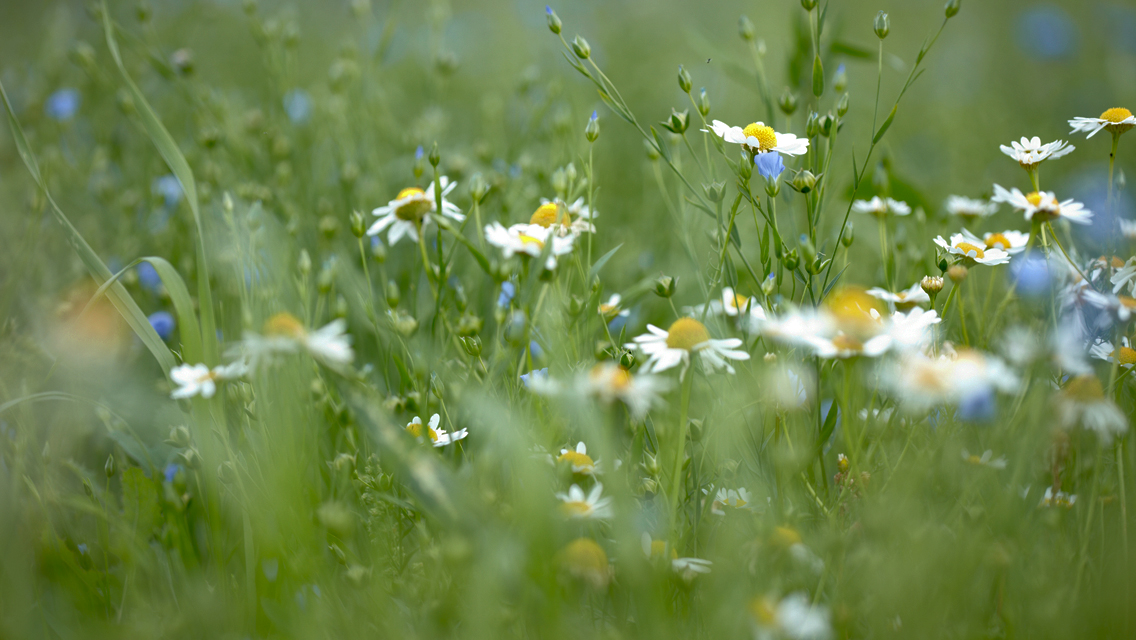
\includegraphics[width = .8\textwidth]{Daisy.jpg}|插入的\texttt{.jpg}格式图档。
\begin{figure}
[htbp]
\centering
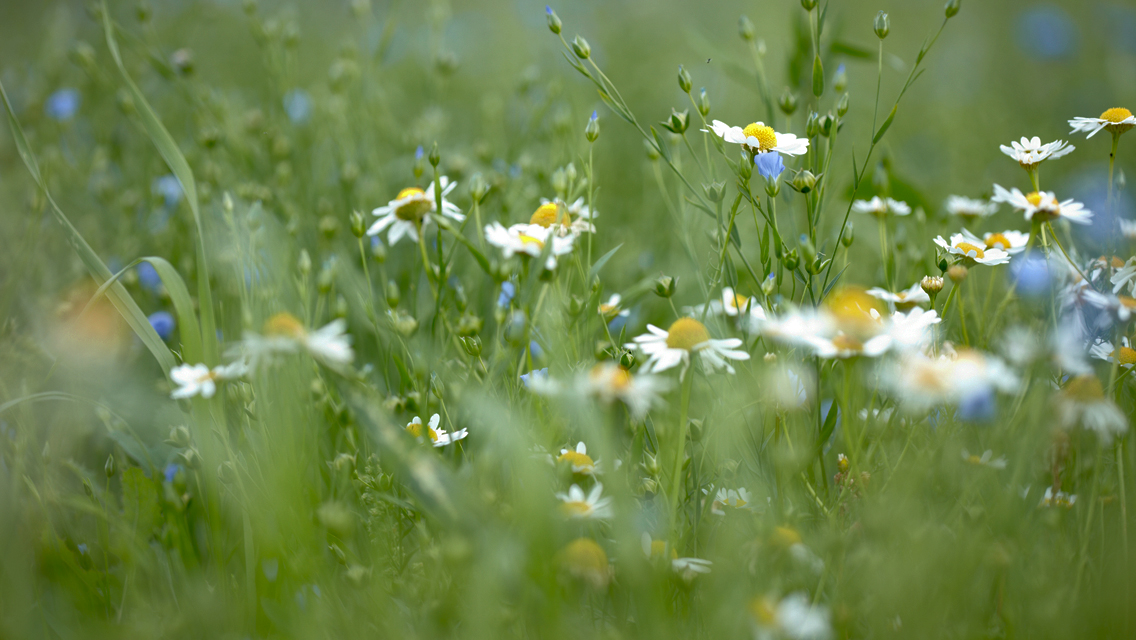
\includegraphics[width = .8\textwidth]{Daisy.jpg}
\caption{一个彩色 \emph{jpg} 图片的例子}\label{Fig:jpg}
\end{figure}

建议使用标准的“三线表”代替Microsoft Office中常见的表格,充满方框的表格给人以舒服的感觉,很烦很讨厌。例如一个简单的三线表如表\ref{Tab:3lines}所示。
\begin{table}
[htbp]
\centering
\begin{tabular}
{ccc}
\toprule
姓名& 学号& 爱好\\
\hline
Ch'en Meng& 00000001& \LaTeX{}\\
Chen Chiang& 00000002& 收集书籍\\
\bottomrule
\end{tabular}
\caption{三线表的示例}\label{Tab:3lines}
\end{table}
\chapter{其他事项}
这个模板是通过研读黄正华老师为武汉大学硕博学生写的\LaTeX{}模板之后由我重写了全部代码而成的,转载和分发都请随意。\footnote{其实我想说遵循GNU的某某文档来着,但是记不得是什么了,允许我偷懒一下。}

这份说明文档也基本来自于黄正华老师为模板写的说明文档,下面插播黄正华老师的广告。

\begin{compactitem}
\item 插图的制作,建议 pgf。 pgf 的长处是源文件直接植入 TEX 文档,管理起来非常方
便。这里有黄正华老师写的一个关于初次使用 pgf 的帖子:\\
\url{http://bbs.ctex.org/forum.php?mod=viewthread&tid=30480}
\item 生成参考文献,建议使用 \BibTeX{}。这里有黄正华老师写的一个文档:\\
\url{http://www.ctex.org/forums/index.php?showtopic=26056}\\
\textit{使用 \BibTeX{} 做参考文献时,借助 EndNote 或者 NoteExpress,可以非常漂亮简
单地解决 bib 文件的录入问题。NoteExpress 在校图书馆网站有正版软件提供下
载。当然 EndNote 本身就是 Thomson Corporation 推出的 (和 SCI 搜索引擎是
同一家公司),和多个重要文献搜索引擎有良好的功能配合。}\\
\textit{Google 学术搜索也提供了文献的 bib 格式。录入参考文献时,偶尔用一用 Google
学术搜索,还可以核查或减少录入的错误,并减少录入的工作量。}
\item 幻灯片的制作,建议使用 Beamer。这里有黄正华老师写的一个模板,供参考:\\
\url{http://www.ctex.org/forums/index.php?showtopic=27695}
\end{compactitem}
\chapter{山东大学研究生院关于学位论文的格式要求}
因为没有找到关于学士学位论文的格式要求,这里附上一段研究生院的要求,仅供参考。
\section{学位论文的基本要求}
硕士学位论文一般应用中文撰写,提倡并鼓励用中、外文撰写。理学、工学、医学类博士学位论文须用中、外文撰写,人文社科类博士学位论文提倡并鼓励用中、外撰写。博士学位论文字数一般3--10万字,摘要为3000字以上;硕士学位论文字数一般2--5万字,摘要为1000字左右。
\section{学位论文的结构要求}
博士、硕士学位论文一般应由以下几部分组成,依次为:
\begin{inparaenum}
\item 论文封面;\item 扉页;\item 原创性声明和关于论文使用授权的声明;\item 中、外文论文目录;\item 中文摘要;\item 外文摘要;\item 符号说明;\item 论文正文(包括文献综述);\item 附录、附图表;\item 引文出处及参考文献;\item 致谢;\item 攻读学位期间发表的学术论文目录;\item 学位论文评阅及答辩情况;\item 外文论文。
\end{inparaenum}
\section{学位论文的格式要求}
\subsection{论文封面}
采用研究生院统一印制的封面。封面的论文题目需要中、外文标示。用小二号加重黑体字打印封面的中文论文题目,用三号加重打印封面外文论文题目,四号加重黑体字打印脊背处论文题目和封面作者姓名、专业、指导教师、合作导师姓名和专业技术职务、论文完成时间、密级、学校代码、学号、分类号等内容。论文题目不得超过30个汉字。分类号须采用《中国图书资料分类法》进行标注。
\subsection{扉页}
论文设扉页,其内容与封面相同,送交校学位办公室、图书馆和档案馆的论文其扉页由本人用碳素钢笔填写。
\subsection{原创性声明和关于学位论文使用授权的说明}
论文作者和指导教师在向校学位办公室、图书馆、档案馆提交论文时必须在要求签名处签字。
\subsection{论文目录}
论文需要有中外文目录各一份。目录应将文内的章、节标题依次排列,并注明页码。标题应简明扼要。中文的“目录”标题字用小三号加重黑体字打印,目录内容用小四号宋体打印。外文的“目录”标题字用加重小三号字体大写字母打印,目录内容用小四号字体小写字母打印。
\subsection{中文摘要}
中文摘要应以最简洁的语言介绍论文的内容要点,其中包括研究目的、研究方法、结果、结论及意义等,并注意突出论文中的新论点、新见解或创造性的成果,并在摘要后列出3--5个关键词,之间用分号相隔。关键词应体现论文的主要内容,词组符合学术规范。“中文摘要” 标题字用小三号加重黑体字打印,摘要内容用小四号宋体打印。
\subsection{外文摘要}
外文摘要内容应与中文摘要基本一致,要语句通顺,语法正确,准确反映论文的内容,并在其后列出与中文相对应的外文关键词。“摘要”标题字用加重小三号字体大写字母打印,摘要内容用小四号字体小写字母打印。
\subsection{符号说明}
介绍论文中所用符号表示的意义。
\subsection{论文正文}
正文是学位论文的主体和核心部分。论文应在前言中包含必要的文献综述,并用小标题标明。论文中的计量单位、制图、制表、公式、缩略词和符号必须遵循国家规定的标准。其行文方式和文体的格局,研究生可根据自己研究课题的表达需要不同而变化,灵活掌握。论文题目用小三号黑体字打印,内容用小四号宋体打印,一般每行32--34字,每页29--31行。每页要有页眉,其上居中打印“山东大学博(硕)士学位论文”字样,页码标注在页面低端(页角)外侧。 论文中的章的标题用小三号加重黑体;节的标题用四号加重黑体;目及子目以下的标题用小四号加重黑体打印,标题应简明扼要,体现阐述内容的重点,无标点符号。
\subsection{附录、附图表}
主要列入正文内过分冗长的公式推导,供查读方便所需的辅助性数学工具或表格;重复性数据图表;实验性图片;程序全文及说明等。
\subsection{引文出处及参考文献}
人文社科类学位论文应有详细的引文出处,格式应规范,一般标注于论文每一页的下方或每一章节的结尾位置。参考文献按文中使用的顺序列出,并注明文献的作者、题名、刊物(出版社)名称、出版时间、页码等。理学、工学、医学类学位论文按国际惯例执行。
\subsection{致谢}
系对给予各类资助、指导和协助完成研究工作以及提供各种对论文工作有利条件的单位和个人表示的感谢。致谢应实事求是,切忌浮夸之词。
\subsection{攻读学位期间发表的学术论文目录}
按学术论文发表的时间顺序,列出本人在攻读学位期间发表或已录用的主要学术论文清单,包括顺序号、论文题名、刊物名称、卷册号及年月、起止页码、论文署名位次。
\subsection{学位论文评阅及答辩情况}
论文答辩通过后,送校学位办公室、图书馆和档案馆的论文需将学位论文评阅及答辩情况填入《学位论文评阅及答辩情况表》中。
\subsection{外文论文}
\subsubsection{外文论文写作的形式}
可根据本学科的实际选择以下写作形式的其中一种。
\begin{compactenum}
\item 与中文全文在内容和形式上完全一致的外文全文;
\item 两篇以上与学位论文相关的可以在外文期刊上发表(含已发表)的外文论文。
\end{compactenum}
\subsubsection{外语写作的要求}
学位论文外语写作要语句通顺,语法正确,符合该种语言的写作规范,能准确反映作者的学术思想。论文内容用小四号字体小写字母打印。
\section{学位论文的打印与装订}
论文用A4标准纸输出,双面打印。博士学位论文一式25份,硕士学位论文一式15份,装订成册,并按要求送交有关部门(送校图书馆和档案馆的论文需线装)。中、外文学位论文原则上一起装订,如篇幅过长可分别装订。除外语专业的学位论文外,其它学科的学位论文一律中文论文在前,外文论文在后。
\vfill
\hfill\begin{minipage}{.3\textwidth}
山东大学研究生院

二〇〇六年十一月十日
\end{minipage}
\chapter{增强这个模板}
欢迎你将你的反馈发送到我的邮箱,\href{mailto:chenmeng0518+TeX@gmail.com}{chenmeng0518+TeX@gmail.com}. 请注意这并不是一个负责回答问题的邮箱。

若是你有兴趣和我一起增强这个模板的功能,也欢迎通过上述邮箱联系我。
